% UCL Thesis LaTeX Template
%  (c) Ian Kirker, 2014
% 
% This is a template/skeleton for PhD/MPhil/MRes theses.
%
% It uses a rather split-up file structure because this tends to
%  work well for large, complex documents.
% We suggest using one file per chapter, but you may wish to use more
%  or fewer separate files than that.
% We've also separated out various bits of configuration into their
%  own files, to keep everything neat.
% Note that the \input command just streams in whatever file you give
%  it, while the \include command adds a page break, and does some
%  extra organisation to make compilation faster. Note that you can't
%  use \include inside an \include-d file.
% We suggest using \input for settings and configuration files that
%  you always want to use, and \include for each section of content.
% If you do that, it also means you can use the \includeonly statement
%  to only compile up the section you're currently interested in.
% You might also want to put figures into their own files to be \input.

% For more information on \input and \include, see:
%  http://tex.stackexchange.com/questions/246/when-should-i-use-input-vs-include


% Formatting rules for theses are here: 
%  http://www.ucl.ac.uk/current-students/research_degrees/thesis_formatting
% Binding and submitting guidelines are here:
%  http://www.ucl.ac.uk/current-students/research_degrees/thesis_binding_submission

% This package goes first and foremost, because it checks all 
%  your syntax for mistakes and some old-fashioned LaTeX commands.
% Note that normally you should load your documentclass before 
%  packages, because some packages change behaviour based on
%  your document settings.
% Also, for those confused by the RequirePackage here vs usepackage
%  elsewhere, usepackage cannot be used before the documentclass
%  command, while RequirePackage can. That's the only functional
%  difference as far as I'm aware.
\RequirePackage[l2tabu, orthodox]{nag}


% ------ Main document class specification ------
% The draft option here prevents images being inserted,
%  and adds chunky black bars to boxes that are exceeding 
%  the page width (to show that they are).
% The oneside option can optionally be replaced by twoside if
%  you intend to print double-sided. Note that this is
%  *specifically permitted* by the UCL thesis formatting
%  guidelines.
%
% Valid options in terms of type are:
%  phd
%  mres
%  mphil
%\documentclass[12pt,phd,draft,a4paper,oneside]{ucl_thesis}
\documentclass[12pt,phd,a4paper,oneside]{ucl_thesis}


% Package configuration:
%  LaTeX uses "packages" to add extra commands and features.
%  There are quite a few useful ones, so we've put them in a 
%   separate file.
% -------- Packages --------

% This package just gives you a quick way to dump in some sample text.
% You can remove it -- it's just here for the examples.
\usepackage{blindtext}

% This package means empty pages (pages with no text) won't get stuff
%  like chapter names at the top of the page. It's mostly cosmetic.
\usepackage{emptypage}

% The graphicx package adds the \includegraphics command,
%  which is your basic command for adding a picture.
\usepackage{graphicx}

% The float package improves LaTeX's handling of floats,
%  and also adds the option to *force* LaTeX to put the float
%  HERE, with the [H] option to the float environment.
\usepackage{float}

% The amsmath package enhances the various ways of including
%  maths, including adding the align environment for aligned
%  equations.
\usepackage{amsmath}
\usepackage{amssymb}

% Use these two packages together -- they define symbols
%  for e.g. units that you can use in both text and math mode.
% \usepackage{gensymb}
% \usepackage{textcomp}
% You may also want the units package for making little
%  fractions for unit specifications.
%\usepackage{units}


% The setspace package lets you use 1.5-sized or double line spacing.
\usepackage{setspace}
\setstretch{1.5}

% That just does body text -- if you want to expand *everything*,
%  including footnotes and tables, use this instead:
%\renewcommand{\baselinestretch}{1.5}


% PGFPlots is either a really clunky or really good way to add graphs
%  into your document, depending on your point of view.
% There's waaaaay too much information on using this to cover here,
%  so, you might want to start here:
%   http://pgfplots.sourceforge.net/
%  or here:
%   http://pgfplots.sourceforge.net/pgfplots.pdf
%\usepackage{pgfplots}
%\pgfplotsset{compat=1.3} % <- this fixed axis labels in the version I was using

% PGFPlotsTable can help you make tables a little more easily than
%  usual in LaTeX.
% If you're going to have to paste data in a lot, I'd suggest using it.
%  You might want to start with the manual, here:
%  http://pgfplots.sourceforge.net/pgfplotstable.pdf
%\usepackage{pgfplotstable}

% These settings are also recommended for using with pgfplotstable.
%\pgfplotstableset{
%	% these columns/<colname>/.style={<options>} things define a style
%	% which applies to <colname> only.
%	empty cells with={--}, % replace empty cells with '--'
%	every head row/.style={before row=\toprule,after row=\midrule},
%	every last row/.style={after row=\bottomrule}
%}


% The mhchem package provides chemistry formula typesetting commands
%  e.g. \ce{H2O}
%\usepackage[version=3]{mhchem}

% And the chemfig package gives a weird command for adding Lewis 
%  diagrams, for e.g. organic molecules
%\usepackage{chemfig}

% The linenumbers command from the lineno package adds line numbers
%  alongside your text that can be useful for discussing edits 
%  in drafts.
% Remove or comment out the command for proper versions.
%\usepackage[modulo]{lineno}
% \linenumbers 


% Alternatively, you can use the ifdraft package to let you add
%  commands that will only be used in draft versions
%\usepackage{ifdraft}

% For example, the following adds a watermark if the draft mode is on.
%\ifdraft{
%  \usepackage{draftwatermark}
%  \SetWatermarkText{\shortstack{\textsc{Draft Mode}\\ \strut \\ \strut \\ \strut}}
%  \SetWatermarkScale{0.5}
%  \SetWatermarkAngle{90}
%}


% The multirow package adds the option to make cells span 
%  rows in tables.
\usepackage{multirow}


% Subfig allows you to create figures within figures, to, for example,
%  make a single figure with 4 individually labeled and referenceable
%  sub-figures.
% It's quite fiddly to use, so check the documentation.
%\usepackage{subfig}

% The natbib package allows book-type citations commonly used in
%  longer works, and less commonly in science articles (IME).
% e.g. (Saucer et al., 1993) rather than [1]
% More details are here: http://merkel.zoneo.net/Latex/natbib.php
%\usepackage{natbib}

% The bibentry package (along with the \nobibliography* command)
%  allows putting full reference lines inline.
%  See: 
%   http://tex.stackexchange.com/questions/2905/how-can-i-list-references-from-bibtex-file-in-line-with-commentary
\usepackage{bibentry}

% The isorot package allows you to put things sideways 
%  (or indeed, at any angle) on a page.
% This can be useful for wide graphs or other figures.
%\usepackage{isorot}

% The caption package adds more options for caption formatting.
% This set-up makes hanging labels, makes the caption text smaller
%  than the body text, and makes the label bold.
% Highly recommended.
\usepackage[format=hang,font=small,labelfont=bf]{caption}

% If you're getting into defining your own commands, you might want
%  to check out the etoolbox package -- it defines a few commands
%  that can make it easier to make commands robust.
\usepackage{etoolbox}


% Sets up links within your document, for e.g. contents page entries
%  and references, and also PDF metadata.
% You should edit this!
%%
%% This file uses the hyperref package to make your thesis have metadata embedded in the PDF, 
%%  and also adds links to be able to click on references and contents page entries to go to 
%%  the pages.
%%

% Some hacks are necessary to make bibentry and hyperref play nicely.
% See: http://tex.stackexchange.com/questions/65348/clash-between-bibentry-and-hyperref-with-bibstyle-elsart-harv
\usepackage{bibentry}
\makeatletter\let\saved@bibitem\@bibitem\makeatother
\usepackage[pdftex,hidelinks]{hyperref}
\makeatletter\let\@bibitem\saved@bibitem\makeatother
\makeatletter
\AtBeginDocument{
    \hypersetup{
        pdfsubject={Thesis Subject},
        pdfkeywords={Thesis Keywords},
        pdfauthor={Author},
        pdftitle={Title},
    }
}
\makeatother
    


% And then some settings in separate files.
% These settings are from:
%  http://mintaka.sdsu.edu/GF/bibliog/latex/floats.html

% They give LaTeX more options on where to put your figures, and may
%  mean that fewer of your figures end up at the tops of pages far
%  away from the thing they're related to.

% Alters some LaTeX defaults for better treatment of figures:
% See p.105 of "TeX Unbound" for suggested values.
% See pp. 199-200 of Lamport's "LaTeX" book for details.

%   General parameters, for ALL pages:
\renewcommand{\topfraction}{0.9}	% max fraction of floats at top
\renewcommand{\bottomfraction}{0.8}	% max fraction of floats at bottom

%   Parameters for TEXT pages (not float pages):
\setcounter{topnumber}{2}
\setcounter{bottomnumber}{2}
\setcounter{totalnumber}{4}     % 2 may work better
\setcounter{dbltopnumber}{2}    % for 2-column pages
\renewcommand{\dbltopfraction}{0.9}	% fit big float above 2-col. text
\renewcommand{\textfraction}{0.07}	% allow minimal text w. figs

%   Parameters for FLOAT pages (not text pages):
\renewcommand{\floatpagefraction}{0.7}	% require fuller float pages
% N.B.: floatpagefraction MUST be less than topfraction !!
\renewcommand{\dblfloatpagefraction}{0.7}	% require fuller float pages

% remember to use [htp] or [htpb] for placement,
% e.g. 
%  \begin{figure}[htp]
%   ...
%  \end{figure} % For things like figures and tables
\bibliographystyle{apalike}

   % For bibliographies
\newcommand{\mc}[1]{\mathcal{\#1}}
\newcommand{\omc}[1]{\overline{\mathcal{#1}}}
\newcommand{\mat}[1]{\mathbf{#1}}
\renewcommand{\mat}[1]{\mathbf{#1}}     % For useful shortcuts

% These control how many number sections your subsections will take
%    e.g. Section 2.3.1.5.6.3
%  and how many of those will get put into the contents pages.
\setcounter{secnumdepth}{3}
\setcounter{tocdepth}{3}


\begin{document}

% ^-- This is a dumb trick that works with the bibentry package to let
%  you put bibliography entries whereever you like.
% I used this to put references to papers a chapter's work was 
%  published in at the end of that chapter.
% For more information, see: http://stefaanlippens.net/bibentry

% If you haven't finished making your full BibTex file yet, you
%  might find this useful -- it'll just replace all your
%  citations with little superscript notes.
% Uncomment to use.
%\renewcommand{\cite}[1]{\emph{\textsuperscript{[#1]}}}

% At last, content! Remember filenames are case-sensitive and 
%  *must not* include spaces.
% I may change the way this is done in a future version, 
%  but given that some people needed it, if you need a different degree title 
%  (e.g. Master of Science, Master in Science, Master of Arts, etc)
%  uncomment the following 3 lines and set as appropriate (this *has* to be before \maketitle)
% \makeatletter
% \renewcommand {\@degree@string} {Master of Things}
% \makeatother

\title{Exploiting Symmetries With Equivariant Transition Models}
\author{YBHQ1\\Supervisor: Prof. Caswell Barry}
\department{Computer Science}

\maketitle

\begin{abstract} % 300 word limit
	This report uses Group Convolutions~\cite{cohen2016group} to construct Equivariant networks used to parameterize reinforcement learning agents, which act in symmetric environments. The Group Convolutions enable the symmetries of the environments to be encoded into the networks, enabling superior generalization. On investigation, using equivariant networks provides substantially better sample efficiency for the reinforcement learning agents. When applied to a model-based setting, equivariant transition models demonstrated superior sample efficiency in learning and outperformed conventional multi-layer perceptron architectures on the symmetric environments tested. However, in the experiments with the Dyna model-based algorithm learning transition models online, was unsuccessful.
\end{abstract}


\setcounter{tocdepth}{2}
% Setting this higher means you get contents entries for
%  more minor section headers.

\tableofcontents
\listoffigures
\listoftables


%  \include{introduction}
%  \include{background}
% \include{literaturereview}
\chapter{Experiments}
\section{Motivation}
With the ultimate aim of leveraging equivariance for model-based RL. A series of Experiments were carried out, sequentially, to investigate how to exploit known symmetries in a model based environment.

Model-Based RL, is inherently more complex than Actor-Critic or Value based methods, as not only does a policy need to be learned, but also a model of the environment dynamics must also be learned.

Due to the increased complexity of Model based methods, and the benefit of implementing existing methods, while also providing a baseline for further experimentation a model-free implementation was created.

\section{Baseline}
The baseline that was chosen was a proximal policy optimization agent from PureJaxRL,~\cite{lu2022discovered}. This baseline provides a training framework, that trains a single agent concurrently on multiple environments.

The Training regime is outlined below in pseudo code.
\begin{algorithm}
	\caption{PureJaxRL PPO Agent Training Structure}
	\begin{algorithmic}
		\State Initialize Agent: Actor-Critic $\pi_\theta$, $v_\phi$
		\State Initialize Replay Buffer: $\mathcal{D}$
		\For{Num Updates}
		\State Gain Experience For Num Timestep
		\State Store trajectories: $\mathcal{D}$.append($(S, A, S', R))$
		\State Calculate GAE Estimate From timesteps
		\For{ Num Epochs}
		\State{ Split GAE Estimates into minibatches}
		\State{ Mini-Batch SGD with Adam on $\pi_\theta, v_\phi$}
		\Comment{ See~\ref{alg:PPO} for Losses to optimize}
		\EndFor
		\EndFor
		\State Returns($\mathcal{D}$)

	\end{algorithmic}
\end{algorithm}

\section{Equivariant Actor-Critics}
\subsection{CartPole}

To form an equivariant network to the group structure of CartPole the actor network must be equivariant to both the identity and inversion operator. This report provides structures for equivariant G-CNNs for both Cart-pole and Catch, that can easily be extended to other environments with known discrete symmetries.


In this section, the outline for the network design is described. In the Catch section, a more detailed description of how to extend the procedure to other Groups is outlined.
The Group for Cart-pole contains two unique elements, in both state and action space. In state space the inversion and identity operator $r, e$ are,
\begin{equation}
	\ell^\mathcal{S}_e =
	\begin{pmatrix}
		1 & 0 & 0 & 0 \\
		0 & 1 & 0 & 0 \\
		0 & 0 & 1 & 0 \\
		0 & 0 & 0 & 1 \\
	\end{pmatrix},
	\ell^\mathcal{S}_r =
	\begin{pmatrix}
		-1 & 0  & 0  & 0  \\
		0  & -1 & 0  & 0  \\
		0  & 0  & -1 & 0  \\
		0  & 0  & 0  & -1 \\
	\end{pmatrix}.
\end{equation}
Then the action space, the inversion and identity operator are,
\begin{equation}
	\ell^\mathcal{A}_e =
	\begin{pmatrix}
		1 & 0 \\
		0 & 1 \\
	\end{pmatrix},
	\ell^\mathcal{A}_r =
	\begin{pmatrix}
		0 & 1 \\
		1 & 0 \\
	\end{pmatrix}.
\end{equation}
Thus, to parameterize an equivariant actor network, the network $\pi_\theta$ must satisfy,
\begin{equation}
	\pi_\theta(\ell^\mathcal{S}_e s) = \ell^\mathcal{A}_e \pi_\theta(s),
\end{equation}
\begin{equation}
	\pi_\theta(\ell^\mathcal{S}_r s) = \ell^\mathcal{A}_r \pi_\theta(s),
\end{equation}
Because the operation on the state space is equivariant to odd functions, the actor network, a simple solution is to use a network with only odd operations, i.e. $\tanh$ activation and no biases for all the of the hidden representations. This ensures that the network is equivariant to the inversion operator. Then we use a group convolution layer to map between representations.

The full network can then be thought of as a composition of $f_\theta : \mathcal{S} \rightarrow \mathbb{R}^{|H|}$, an odd embedding MLP and $gc_\theta: \mathbb{R}^{|H|} \rightarrow \mathbb{R}^{\mathcal{A}}$ a group convolution layer that "lifts" the equivariance to the action space. As such the parametric policy is,
\begin{equation}
	\pi_\theta(s) = gc_\theta(f_\theta(s)).
\end{equation}
The non-trivial equivariance properties of the sub-networks are,
\begin{equation}
	f_\theta(-s) = -f_\theta(s),
\end{equation}
\begin{equation}
	gc_\theta(-x) =
	\begin{pmatrix}
		0 & 1 \\
		1 & 0 \\
	\end{pmatrix}
	gc_\theta(x),
\end{equation}
Where $gc_\theta(x) = [P(A=a_0), P(A=a_1)]$ describes the distribution over the binary actions of Cart-pole.

This G-CNN network for policy learning is the first novel contribution of this report. In comparison to the work of \cite{mondal2020group}, the policy learning G-CNN is fully equivariant, rather than learning action values from an equivariant embedding. Additionally, the network parameterizes a policy directly rather than Q values. Due to the network's end to end equivariance in comparison to the Q-value network proposed by \cite{mondal2020group}, agents parameterized by this network must take the same actions in states that are in the same orbit, which is not the case for the Q-value network which only has an equivariant embedding.

Further, this network architecture has advantages over Symmetrizer networks, \cite{vanderpol2020mdp}, in that it does not require a large matrix inversions to solve for the parameters of the network, while still maintaining the same equivariance qualities.

\subsection{Training Dynamics On the Cart-Pole Benchmark}

With the networks structure defined, the benchmark task is to learn an expert policy on the Cart-pole environment. In the default setting Cart-pole has a maximum episode length of 500 interactions. All non-terminal states garner a reward of +1. As such, the maximum episodic return is 500. As in all conventional RL problems, in Cart-pole the aim is to maximize the episodic return of the agent. It is straightforward to find an expert policy in Cart-pole, with conventional deep learning methods, and serves only as an implementation benchmark. For an equivariant network structure to improve the learned policy quality it should approach the goal of 500 episodic return with fewer MDP interactions.

When comparing policy agent's learning dynamics it is not only important that, the agent achieves expertise in the task but also that, the policy learning procedure is stable across many random seeds. Where a random seed is the random initial state that the agent and environment start in. With training stability in mind looking at the worst performing random seeds is informative, as if the algorithm is very sensitive to initialization, then this performance may be heavily affected.

For all the experiments, we leave the critic to be a standard MLP, with no equivariance constraints. This may be a non-optimal setting in terms of performance. Additionally, to ensure that all the agent's learning is stable training is performed across 128 random seeds.

Due to the constraints on the equivariant network structures, it is not always possible to have exactly the same number of parameters exactly in the networks. In cases, where exact parameter count matching all network's depth is held constant and, a width is found such that the parameter counts are inside 10\% less.

Below, in fig\ref{fig:cartpole_equivariant_actor}, the episodic return's of three different agents with differing network architectures are plotted. The network's training hyperparameters are all the same, and are those found in the PureJaxRL\cite{lu2022discovered} baselines. The three networks are an MLP baseline from PureJaxRL, an implementation of the Symmetrizer network from \cite{vanderpol2020mdp}, and this report's G-CNN policy network.
\begin{figure}[H]
	\centering
	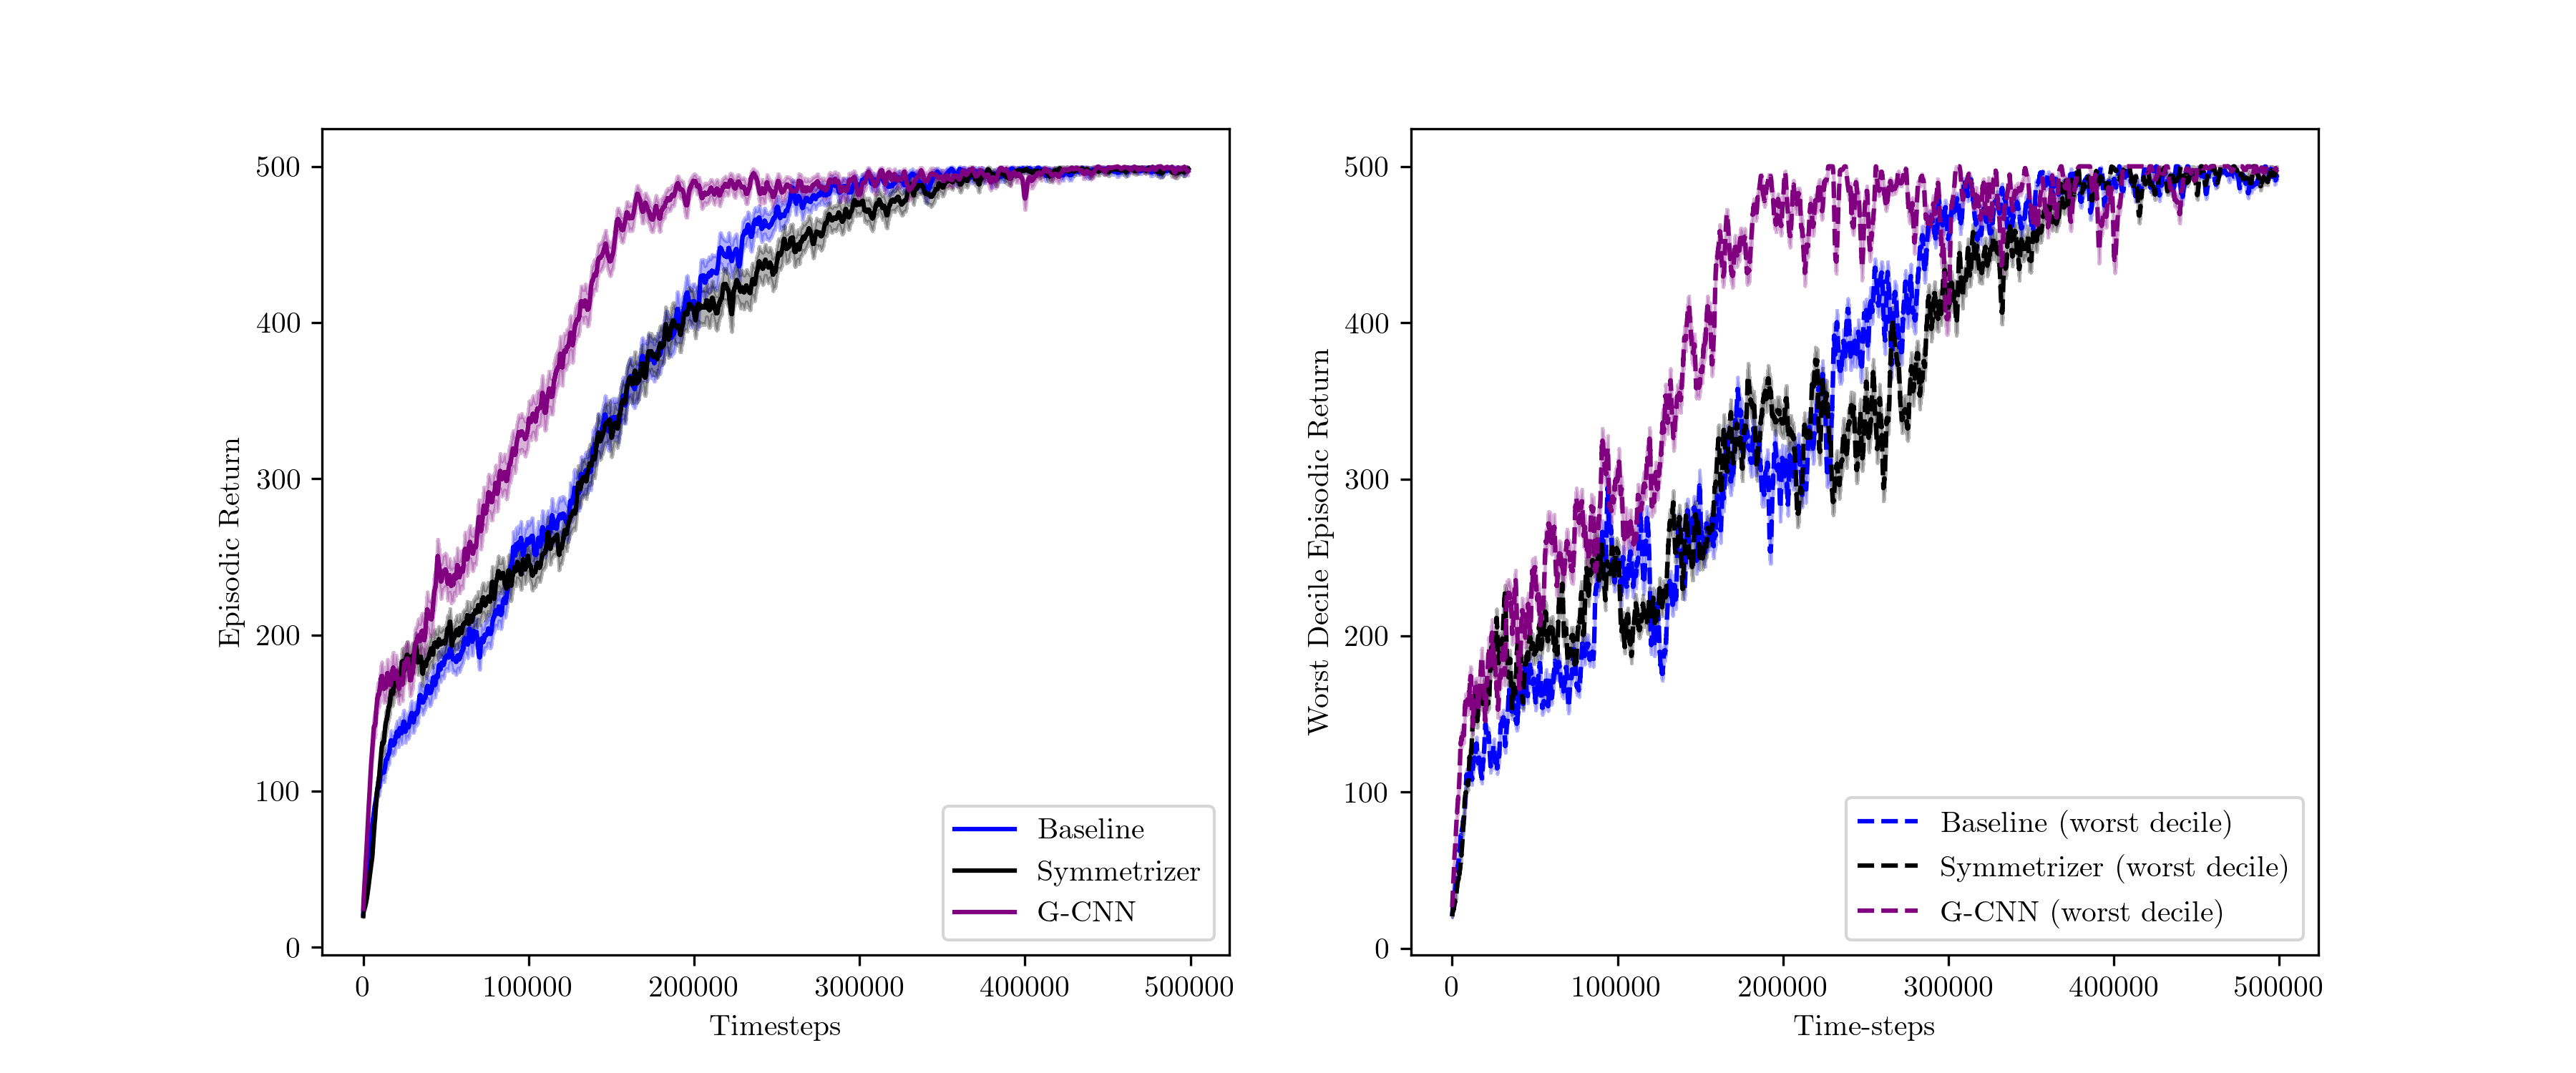
\includegraphics[width=\linewidth]{Figures/cart_pole_returns.png}
	\caption{Left: Mean cumulative episodic returns for the CartPole agents across 128 random seeds plotted against number of experience time-steps in the MDP. Right: The mean cumulative episodic returns of the worst performing 128 random seeds against number of experience time-steps in the MDP. Both of the plots are moving averages, with windows of 10 time-steps. } \label{fig:cartpole_equivariant_actor}
\end{figure}

Both the Symmetrizer and the G-CNN are equivariant to the actions of the $C_2$ group. This equivariance constraint requires a learned policy that respects the inversion symmetry present in Cart-pole. The equivarianc  should improve the sample efficiency of the agent as any learning from one state additionally informs the agent about the agent about the policy for the other state in the orbit. This hypothesis, is supported somewhat by the observed training dynamics. Over the first period of training both the Symmetrizer and the G-CNN, outperform the baseline. The Symmetrizer, does not maintain this performance advantage. Our implementation uses the same network size, as the original paper and the same network hyperparameters. Despite this, the symmetrizer agent fails to learn an expert policy in fewer steps than that of the baseline. The equivariant nature of the network was asserted.

It should be noted that here the mean plus minus two standard deviations is plotted in comparison to the median and upper and lower quartiles of cumulative returns, which is plotted in \cite{vanderpol2020mdp}. The performance of the Symmetrizer, is underwhelming despite the implemented network being checked for equivariance. Further tuning of the hyperparameters may yield performance that improves upon the baseline's returns. However, this was not a primary concern.

The G-CNN does compare favourably with the baseline implementation of an MLP, having slightly fewer parameters. It can be seen that it both converges on average to an expert policy in fewer time-steps but also has a more favourable convergence behaviour in the worst case scenario. This can be seen in the right of Figure \ref{fig:cartpole_equivariant_actor} where, the bottom tenth percentile of cumulative returns, still converges notably faster than that of the baseline.

\begin{table}
	\centering
	\begin{tabular}{|c|c|c|c|}
		\hline
		Time-steps & Baseline     & Symmetrizer  & G-CNN        \\
		\hline
		$10, 000$  & $102 \pm 5$  & $116 \pm 6$  & $158 \pm 8$  \\
		$100, 000  & $260 \pm 10$ & $240 \pm$ 10 & $330 \pm 10$ \\
		$500,000$  & $497 \pm 1$  & $500 \pm 1$  & $499 \pm 1$  \\
		\hline
	\end{tabular}
	\caption{Cumulative episodic returns tabulated for the three network architectures. All episodic returns are recorded with confidence intervals of two standard errors across 128 random seeds.}
\end{table}











% \chapter{My First Content Chapter}
\label{chapterlabel2}

% This just dumps some pseudolatin in so you can see some text in place.
\blindtext

% \section{Notes}

\textbf{Definition: MDP Homomorphism} Given some MDP $\mathcal{M}$, where there
exists a surjective map, from $\mathcal{S} \times \mathcal{A} \rightarrow \omc{S} \times
	\omc{A}$. the MDP $\omc{M}$ is an abstract MDP over the new space. The
homomorphism $h$, then is the tuple of $(\sigma, \alpha_s|s \in \mathcal{S})$, where
$\sigma: \mathcal{S} \rightarrow \omc{S}$ and $\alpha_s : \mathcal{A} \rightarrow \omc{A}$.
This surjective map must satisfy two constraints for it to be a valid MDP
homomorphism; \begin{enumerate} \item $R(s, a) = R(\sigma(s), \alpha_s(a))$
	\item $T(s', a, s) = T(\sigma(s'), \alpha_s(a), \sigma(s))$ \end{enumerate}


Rather than learning a tranditional MDP homomorphism, we wish to learn a homomorphic map

$$h: \mathcal{A} \times \mathcal{S} \times \overline{\mathcal{A}} -> \omc{S}$$

With the constraints that the homomorphsim in the simplest case maps of invertersion symmetry $D_2$ where in state space the $D_2$ representtion is $L_2$ and in action space the $D_2$ representaiton is $K_2$. so that $$h(a, s, \overline{a}) = h(K_2 a, L_2 s, \overline{a})$$.

Because we are learning from determinsistic dynamics $T: \mathcal{S} \times \mathcal{A} \rightarrow \mathcal{S}$ and $\overline{T}: \omc{S} \times \omc{A} \rightarrow \omc{S}$ we must also learn that

$$\overline{T}(\overline{s}, \overline{a}) = h(T(s, a), a', \overline{a})$$.

where $overline{s} = h(s, a, \overline{a})$

$$\overline{T}(h(s, a, \overline{a}), \overline{a}) = h(T(s, a), a', \overline{a})$$.


In the case of the cartpole the actions $a, \overline{a} \in [0, 1]$.


\subsection{Training}
The objectiive of training is to use some kind of similarity metric like that used in Approximate MDP Homomorphisms to learn the parametric form of $h$ in a supervised setting, over these (state, action, abstract action, next state) tuples.
With the hypothesis that having a group equivariant network will make the learning more efficient.

% \chapter{General Conclusions}
\label{chapterlabel4}

% This just dumps some pseudolatin in so you can see some text in place.
\blindtext

% \addcontentsline{toc}{chapter}{Appendices}

% The \appendix command resets the chapter counter, and changes the chapter numbering scheme to capital letters.
%\chapter{Appendices}
\appendix
\chapter{An Appendix About Stuff}
\label{appendixlabel1}
(stuff)

\chapter{Another Appendix About Things}
\label{appendixlabel2}
(things)

\chapter{Colophon}
\label{appendixlabel3}
\textit{This is a description of the tools you used to make your thesis. It helps people make future documents, reminds you, and looks good.}

\textit{(example)} This document was set in the Times Roman typeface using \LaTeX\ and Bib\TeX , composed with a text editor. 
 % description of document, e.g. type faces, TeX used, TeXmaker, packages and things used for figures. Like a computational details section.
% e.g. http://tex.stackexchange.com/questions/63468/what-is-best-way-to-mention-that-a-document-has-been-typeset-with-tex#63503

% Side note:
%http://tex.stackexchange.com/questions/1319/showcase-of-beautiful-typography-done-in-tex-friends

% You could separate these out into different files if you have
%  particularly large appendices.

% This line manually adds the Bibliography to the table of contents.
% The fact that \include is the last thing before this ensures that it
% is on a clear page, and adding it like this means that it doesn't
% get a chapter or appendix number.
\addcontentsline{toc}{chapter}{Bibliography}
% Actually generates your bibliography.

\bibliography{bibliography}
% All done. \o/
\end{document}
